\chapter{Projeto e Arquitetura do Sistema}
\label{ch:arquitetura}

Neste capítulo descreve-se o projeto do sistema: a arquitetura geral, a estrutura mecânica, o hardware e o esquema elétrico, o software e a organização dos módulos. As escolhas resultam da análise feita no capítulo~\ref{ch:estado-arte} e dos requisitos do capítulo~\ref{ch:introducao}. Os valores apresentados (pinos, frequências, limites) constituem a proposta inicial e serão confirmados durante a implementação.

\section{Arquitetura geral}
A figura~\ref{fig:blocos} mostra o diagrama de blocos do sistema. O telemóvel envia, por Bluetooth, a inclinação pretendida e os comandos de modo. O módulo Bluetooth converte a ligação sem fios numa porta série, lida pelo microcontrolador. O microcontrolador lê a \gls{imu} fixa à plataforma, estima a atitude, calcula os comandos e gera os sinais \gls{pwm} dos dois servos. A alimentação é feita por uma bateria, com um regulador dedicado aos servos e outro à eletrónica.

\begin{figure}[H]
\centering
\begin{tikzpicture}[scale=0.85, transform shape,
  bloco/.style={draw, rounded corners=2pt, minimum width=2.5cm, minimum height=1cm, align=center, font=\small},
  pot/.style={bloco, fill=orange!15},
  sinal/.style={-{Latex[length=2mm]}, thick},
  energia/.style={-{Latex[length=2mm]}, thick, orange!80!black, dashed},
  lab/.style={font=\scriptsize}]
\node[bloco, fill=gray!10] (tel) at (-2.3,0) {Telemóvel\\(app)};
\node[bloco] (bt) at (1.9,0) {Módulo Bluetooth\\modo duplo};
\node[bloco, fill=blue!8, minimum height=2.2cm] (mcu) at (6.2,0) {NUCLEO-\\F767ZI};
\node[bloco] (imu) at (6.2,2.7) {\acrshort{imu} GY-85\\(plataforma)};
\node[bloco, fill=gray!10] (pc) at (1.9,2.7) {PC (registo)};
\node[bloco] (s1) at (10.8,0.75) {Servo \textit{roll}\\MG996R};
\node[bloco] (s2) at (10.8,-0.75) {Servo \textit{pitch}\\MG996R};
\node[pot] (reg5) at (6.2,-3.0) {Regulador \SI{5}{\volt}};
\node[pot] (ubec) at (10.8,-3.0) {\acrshort{ubec} \SI{6}{\volt}\\$\geq$\SI{5}{\ampere}};
\node[pot] (bat) at (6.2,-5.0) {Bateria LiPo 2S\\+ fusível};
\node[bloco, fill=red!10] (es) at (10.8,-5.0) {Paragem de\\emergência};

\draw[sinal, <->] (tel) -- node[above, lab]{Bluetooth} (bt);
\draw[sinal, <->] ($(bt.east)+(0,-0.2)$) -- node[below, lab]{\acrshort{uart}} ($(mcu.west)+(0,-0.2)$);
\draw[sinal, <->] (imu) -- node[right, lab]{\acrshort{i2c}} (mcu);
\draw[sinal, <->] (pc.south) |- node[pos=0.75, above, lab]{USB (ST-LINK)} ($(mcu.west)+(0,0.75)$);
\draw[sinal] (mcu.east |- s1) -- node[above, lab]{\acrshort{pwm}} (s1);
\draw[sinal] (mcu.east |- s2) -- node[below, lab]{\acrshort{pwm}} (s2);
\draw[sinal] ($(es.west)+(0,0.25)$) -- ++(-0.6,0) |- node[pos=0.75, above, lab]{contacto auxiliar} (8.3,-1.8) -| ($(mcu.south east)+(-0.4,0)$);
\draw[energia] (bat) -- (reg5);
\draw[energia] (reg5) -- (mcu);
\draw[energia] (bat.east) -- ++(0.9,0) |- ($(es.west)+(0,-0.3)$);
\draw[energia] (es) -- (ubec);
\draw[energia] (ubec) -- (s2);
\draw[energia] (ubec.east) -- ++(0.45,0) |- (s1.east);
\end{tikzpicture}
\caption{Diagrama de blocos do sistema (sinal a cheio, energia a tracejado).}
\label{fig:blocos}
\end{figure}

O sistema tem dois modos de funcionamento previstos. No modo de seguimento, a referência é a inclinação do telemóvel; no modo de nivelamento, a referência é a horizontal e o controlador compensa o movimento da base. Em ambos os casos o controlo é executado localmente, pelo que uma falha da ligação Bluetooth nunca deixa a plataforma sem controlo (RNF6).

\section{Estrutura mecânica}
A estrutura foi modelada em OpenSCAD, de forma paramétrica, e é composta por quatro peças impressas em 3D: a caixa, a tampa com as torres, o quadro do eixo de \textit{roll} e a plataforma do eixo de \textit{pitch} (figuras~\ref{fig:cad-montagem} e~\ref{fig:cad-explodida}). Segue a solução de \textit{gimbal} em série usada nos estabilizadores de câmara: o servo de \textit{roll} está fixo à tampa e roda o quadro, e o servo de \textit{pitch} está fixo ao quadro e roda a plataforma. Os dois eixos cruzam-se no mesmo ponto, \SI{70}{\milli\metre} acima da tampa, pelo que cada servo atua num só ângulo e não há acoplamento mecânico entre eixos.

\begin{figure}[H]
\centering
\begin{subfigure}[b]{0.48\textwidth}
\centering
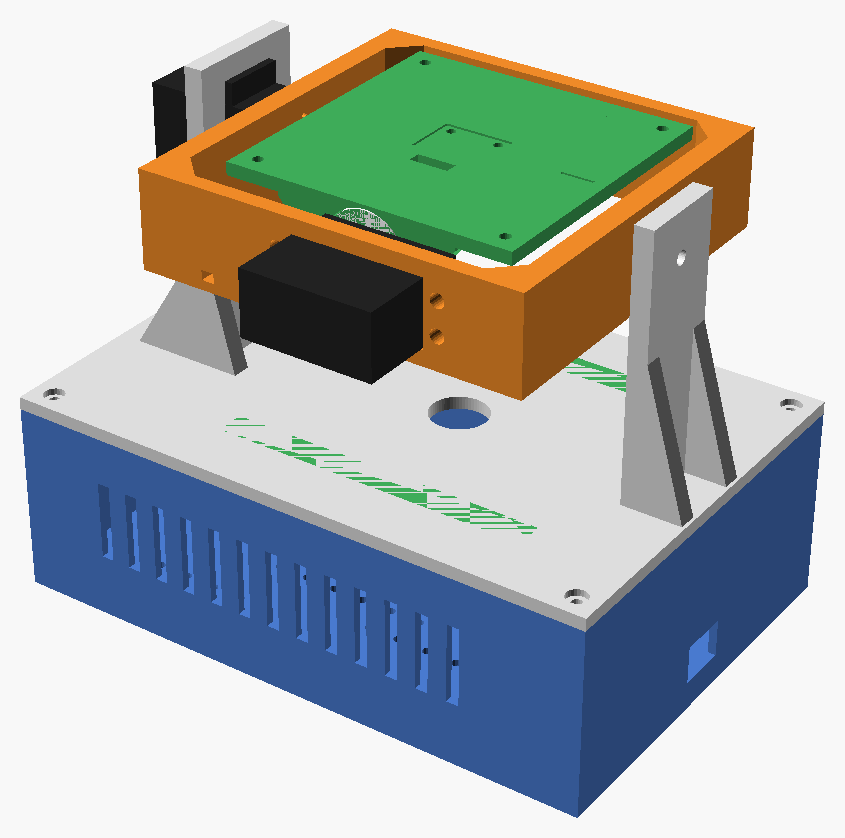
\includegraphics[width=\textwidth]{figuras/montagem.png}
\caption{Posição neutra}
\end{subfigure}\hfill
\begin{subfigure}[b]{0.48\textwidth}
\centering
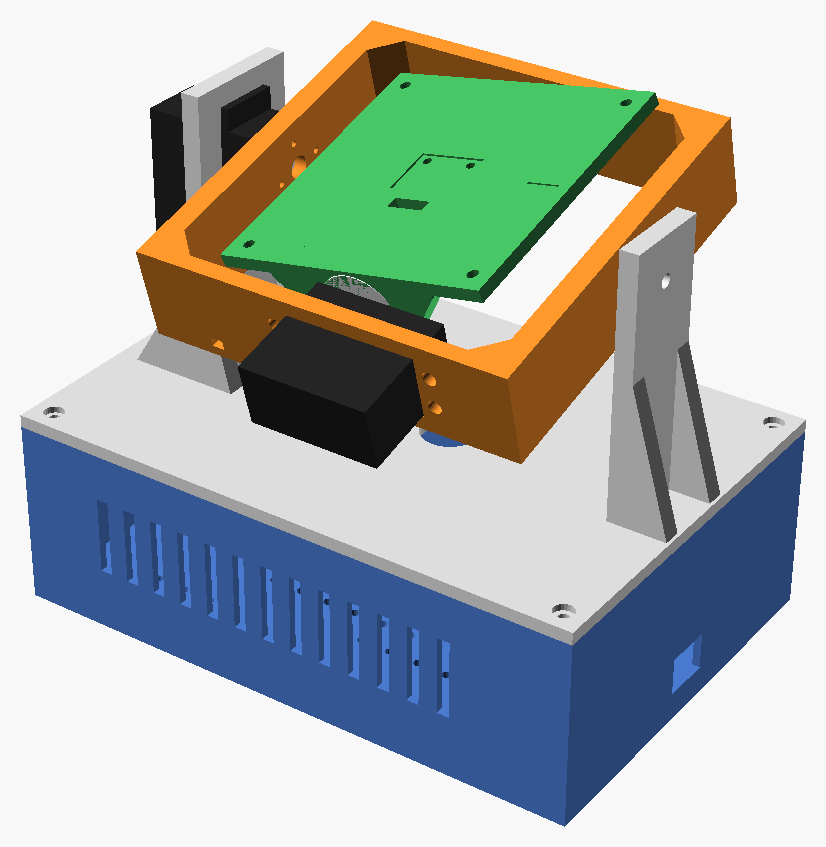
\includegraphics[width=\textwidth]{figuras/montagem_inclinada.png}
\caption{\textit{Roll} de \SI{15}{\degree} e \textit{pitch} de \SI{-12}{\degree}}
\end{subfigure}
\caption{Modelo 3D da plataforma montada (OpenSCAD).}
\label{fig:cad-montagem}
\end{figure}

\begin{figure}[H]
\centering
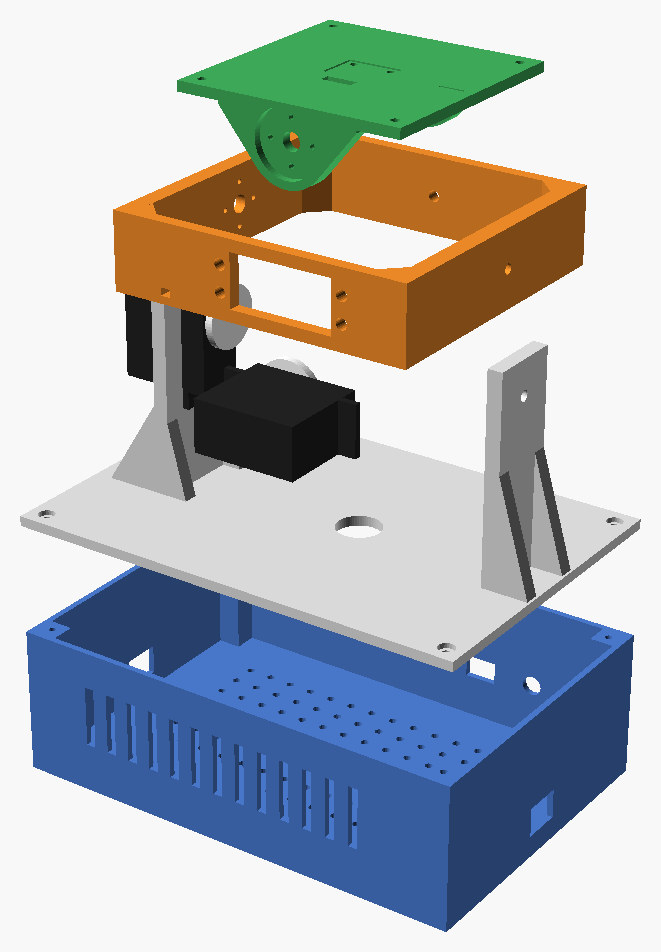
\includegraphics[width=0.55\textwidth]{figuras/explodida.png}
\caption{Vista explodida: caixa (azul), tampa com torres (cinzento), quadro de \textit{roll} (laranja), plataforma de \textit{pitch} (verde) e servos (preto).}
\label{fig:cad-explodida}
\end{figure}

Cada eixo é suportado nos dois lados. Num lado, a peça móvel é aparafusada ao disco (\textit{horn}) do servo, de \SI{25}{\milli\metre} de diâmetro, encaixado num rebaixo de \SI{3}{\milli\metre} e fixo com quatro parafusos M2. No lado oposto, um parafuso M4 funciona como pivô, com uma porca embutida na peça móvel e uma anilha para garantir a folga axial. Assim, o servo não suporta sozinho o peso da peça que roda, o que reduz o esforço no seu veio.

\begin{figure}[H]
\centering
\begin{subfigure}[b]{0.48\textwidth}
\centering
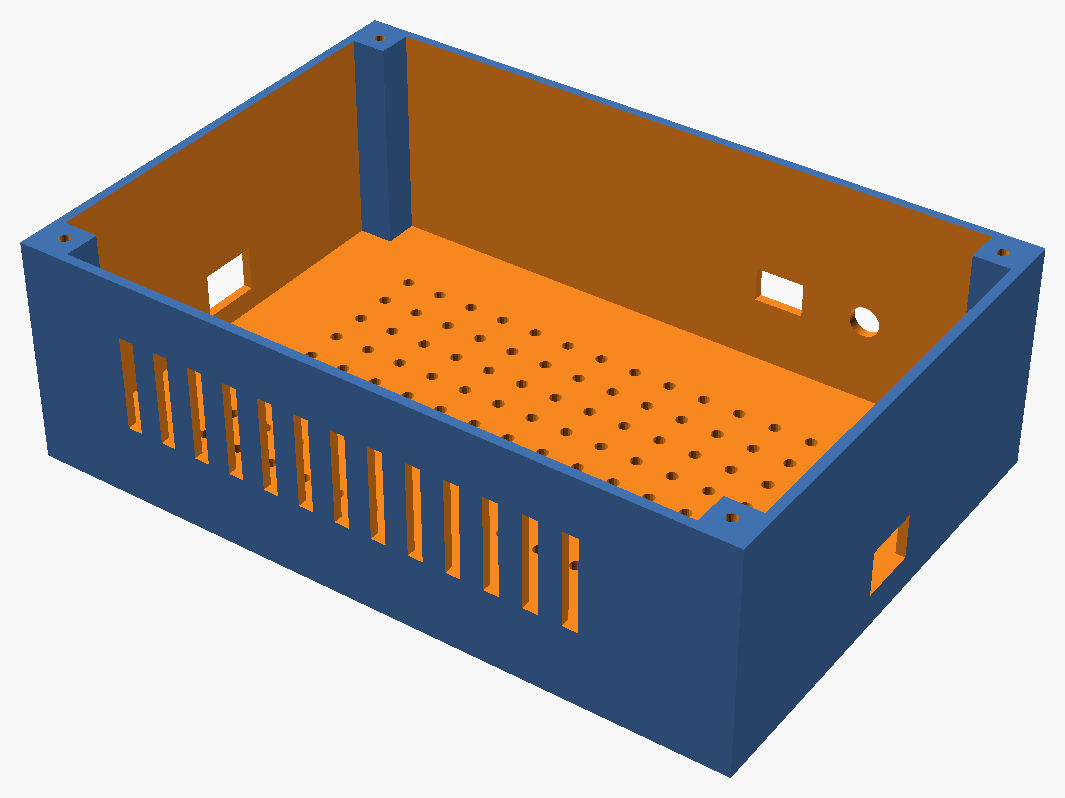
\includegraphics[width=\textwidth]{figuras/peca_caixa.png}
\caption{Caixa}
\end{subfigure}\hfill
\begin{subfigure}[b]{0.48\textwidth}
\centering
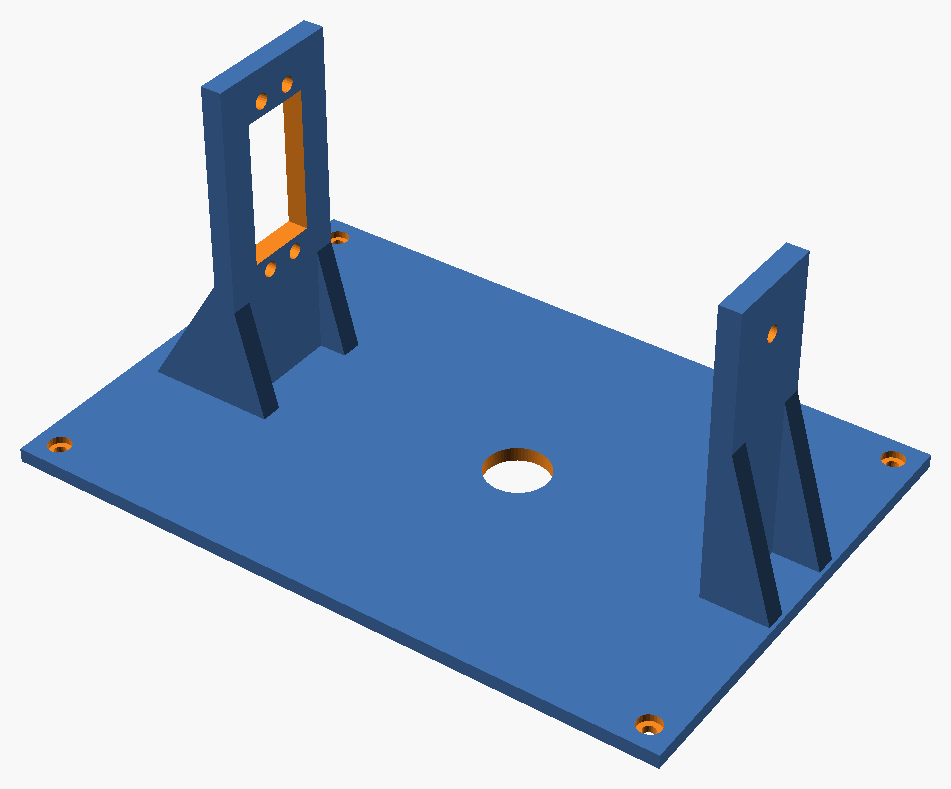
\includegraphics[width=\textwidth]{figuras/peca_tampa.png}
\caption{Tampa com torres}
\end{subfigure}
\\[2mm]
\begin{subfigure}[b]{0.48\textwidth}
\centering
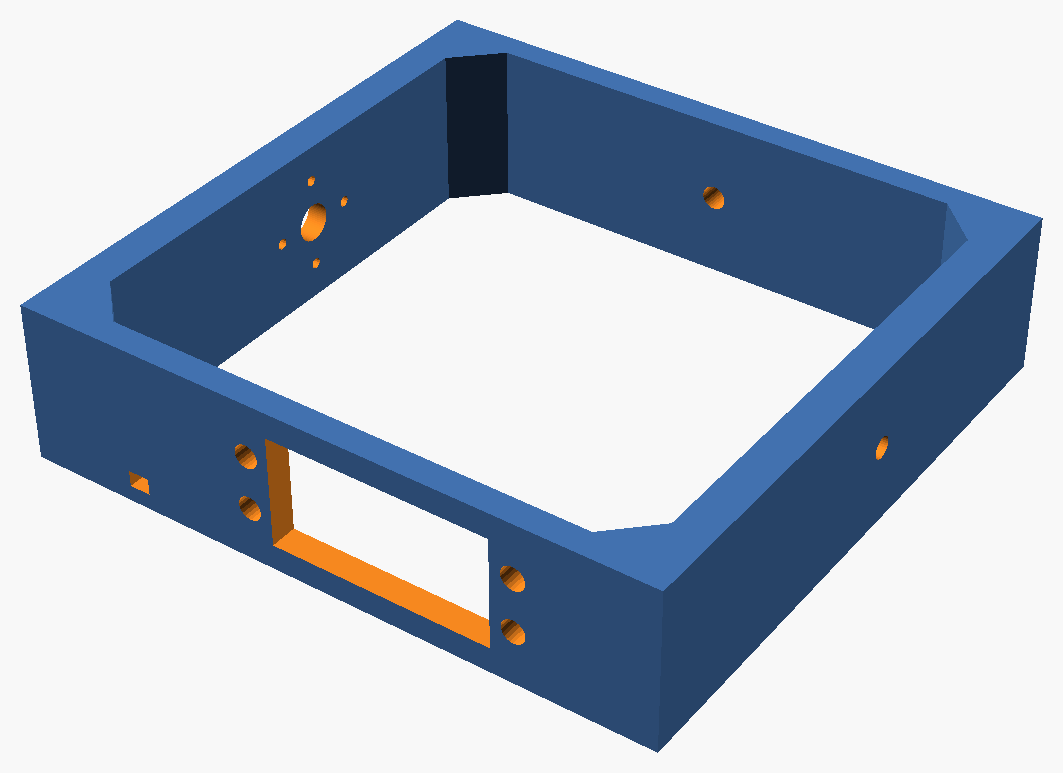
\includegraphics[width=\textwidth]{figuras/peca_quadro.png}
\caption{Quadro do eixo de \textit{roll}}
\end{subfigure}\hfill
\begin{subfigure}[b]{0.48\textwidth}
\centering
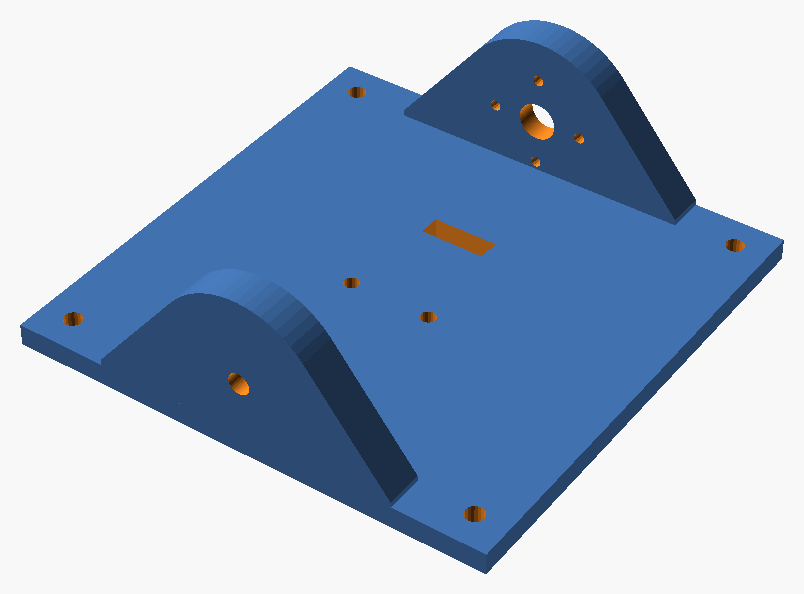
\includegraphics[width=\textwidth]{figuras/peca_plataforma.png}
\caption{Plataforma do eixo de \textit{pitch}}
\end{subfigure}
\caption{Peças impressas em 3D, na orientação de impressão.}
\label{fig:cad-pecas}
\end{figure}

A tabela~\ref{tab:pecas} resume as peças e as suas funções.

\begin{table}[H]
\centering\small
\caption{Peças da estrutura mecânica.}
\begin{tabularx}{\textwidth}{>{\raggedright\arraybackslash}p{2.6cm}>{\raggedright\arraybackslash}p{3.4cm}Y}
\toprule
Peça & Dimensões principais & Função e detalhes\\\midrule
Caixa & $190\times130\times\SI{60}{\milli\metre}$; parede de \SI{2.5}{\milli\metre} & Aloja a NUCLEO, os módulos, os reguladores e a bateria. Fundo com grelha de furos M3 a cada \SI{10}{\milli\metre} para fixar as placas; aberturas para os dois USB da NUCLEO, para a ficha de alimentação e para o interruptor; ranhuras de ventilação\\
Tampa e torres & Tampa de \SI{4}{\milli\metre}; eixos a \SI{70}{\milli\metre} & Torre do servo de \textit{roll} e torre do pivô, com nervuras de reforço; furos de passagem dos cabos; fixação à caixa por quatro parafusos M3\\
Quadro (\textit{roll}) & Moldura de $120\times\SI{115}{\milli\metre}$, paredes de 5 a \SI{7}{\milli\metre} & Ligado ao \textit{horn} do servo de \textit{roll} e ao pivô; transporta o servo de \textit{pitch}; passagem para braçadeira do cabo\\
Plataforma (\textit{pitch}) & $90\times90\times\SI{4}{\milli\metre}$ & Ligada ao \textit{horn} do servo de \textit{pitch} e ao pivô; rebaixo central para a \acrshort{imu}; furos M3 nos cantos para fixar carga; marcação do eixo $x$\\
\bottomrule
\end{tabularx}
\label{tab:pecas}
\end{table}

O modelo usa uma folga de impressão de \SI{0.3}{\milli\metre} e as cotas do MG996R estão parametrizadas, devendo ser confirmadas com paquímetro antes da impressão. O rebaixo da \gls{imu} na plataforma foi desenhado para o módulo GY-521 ($21{,}5\times\SI{16.5}{\milli\metre}$). O GY-85 tem dimensões muito próximas (cerca de $22\times\SI{17}{\milli\metre}$) \cite{gy85}, mas a posição dos furos de fixação tem de ser verificada e ajustada no modelo.

\section{Arquitetura de hardware}

\subsection{Unidade de processamento}
A NUCLEO-F767ZI é alimentada a \SI{5}{\volt} por um regulador dedicado, através da entrada E5V, ou, durante o desenvolvimento, pelo USB do ST-LINK. O ST-LINK disponibiliza também uma porta série virtual, usada para enviar dados de registo para o PC durante os ensaios.

\subsection{Sensor inercial}
O módulo GY-85 é ligado ao barramento \gls{i2c}1 a \SI{400}{\kilo\hertz}. Os três circuitos partilham o barramento, com endereços distintos: ADXL345 em 0x53, ITG-3205 em 0x68 ou 0x69 e HMC5883L em 0x1E \cite{gy85datasheet}. O primeiro teste (IMU-01) é um varrimento do barramento para confirmar os endereços da placa usada.

Propõe-se configurar o acelerómetro em modo de resolução total, na gama de $\pm\SI{2}{g}$, que chega para medir a inclinação, e o giroscópio na gama de $\pm\SI{2000}{\degree\per\second}$, com o filtro passa-baixo digital interno ativo para reduzir o ruído das vibrações dos servos. O magnetómetro não é usado no controlo, mas é configurado para ficar disponível. A leitura é feita por \textit{polling}, sincronizada com o ciclo de \SI{200}{\hertz}.

\subsection{Atuadores}
Os dois servos MG996R são comandados por dois canais do mesmo temporizador, a \SI{50}{\hertz}. Com o relógio do temporizador dividido para \SI{1}{\mega\hertz}, cada unidade corresponde a \SI{1}{\micro\second}, o que dá uma resolução muito superior à banda morta do servo (\SI{5}{\micro\second}) \cite{mg996r}. A largura de impulso é limitada em software a uma janela calibrada, de modo a nunca forçar os batentes mecânicos.

\subsection{Comunicação}
O módulo Bluetooth de modo duplo (HM-12) liga-se à USART6 do microcontrolador \cite{hm12}. Funciona a 9600~bps por omissão. Uma mensagem de referência tem cerca de 25 bytes, o que a esta velocidade ocupa cerca de \SI{26}{\milli\second}; a \SI{20}{\hertz} o canal fica ocupado a cerca de metade. Se o módulo o permitir, a velocidade será aumentada por comando AT para dar margem.

\subsection{Alimentação}
A alimentação é feita por uma bateria LiPo 2S (\SI{7.4}{\volt} nominais, \SI{8.4}{\volt} carregada), protegida por um fusível logo à saída e com um interruptor geral. Os servos são alimentados por um \gls{ubec} de \SI{6}{\volt}, separado da eletrónica para que os picos de corrente não perturbem o microcontrolador nem a \gls{imu}. Como cada MG996R pode consumir \SI{2.5}{\ampere} em bloqueio, o regulador deve fornecer pelo menos \SI{5}{\ampere}; um \gls{ubec} de \SI{3}{\ampere} \cite{hobbywingubec} só serve se o software impedir que os dois servos fiquem bloqueados em simultâneo. Junto aos servos coloca-se um condensador eletrolítico de \SI{1000}{\micro\farad} para absorver os picos. Todas as massas são ligadas num ponto comum.

A tensão da bateria é medida por um divisor resistivo ligado a uma entrada analógica. Com $R_1 = \SI{10}{\kilo\ohm}$ e $R_2 = \SI{4.7}{\kilo\ohm}$, os \SI{8.4}{\volt} da bateria carregada correspondem a \SI{2.69}{\volt} no \gls{adc}, abaixo do limite de \SI{3.3}{\volt}.

A paragem de emergência é um botão com dois contactos normalmente fechados. O primeiro está em série com a alimentação dos servos e corta-a fisicamente quando o botão é atuado. O segundo liga uma entrada digital à massa: em funcionamento normal a entrada lê 0; com o botão atuado o contacto abre, a resistência interna de \textit{pull-up} leva a entrada a 1 e o microcontrolador passa ao estado de falha.

\begin{table}[H]
\centering\small
\caption{Balanço energético estimado.}
\begin{tabularx}{\textwidth}{>{\raggedright\arraybackslash}p{4cm}YYY}
\toprule
Carga & Tensão & Corrente típica & Corrente de pico\\\midrule
2 servos MG996R & \SI{6}{\volt} & \SI{0.5}{\ampere} (total, estimado) & \SI{5}{\ampere} (bloqueio)\\
NUCLEO-F767ZI + \acrshort{imu} + Bluetooth & \SI{5}{\volt} & \SI{0.35}{\ampere} (estimado) & \SI{0.5}{\ampere}\\
\midrule
Potência média & \multicolumn{3}{p{9cm}}{$\approx \SI{3}{\watt} + \SI{1.75}{\watt} \approx \SI{4.8}{\watt}$; cerca de \SI{5.6}{\watt} à saída da bateria, com rendimento de 85\,\% nos reguladores}\\
\bottomrule
\end{tabularx}
\label{tab:energia}
\end{table}

Uma bateria de \SI{2200}{\milli\ampere\hour} armazena cerca de \SI{16}{\watt\hour}. Usando apenas 80\,\% dessa energia, a autonomia estimada é de $16 \times 0{,}8 / 5{,}6 \approx \SI{2.3}{\hour}$, bem acima dos \SI{30}{\minute} do requisito RNF7. As correntes típicas são estimativas e serão medidas no ensaio T-ALIM.

\section{Esquema elétrico}
O esquema elétrico está dividido em duas partes: as ligações de sinal entre a NUCLEO e os módulos (figura~\ref{fig:esq-sinal}) e o circuito de alimentação (figura~\ref{fig:esq-alim}). Nas figuras, os nomes \texttt{+5V}, \texttt{+6V\_SERVO}, \texttt{VBAT\_ADC} e GND indicam ligações à mesma rede. A tabela~\ref{tab:pinos} resume os pinos usados.

\begin{figure}[H]
\centering
\begin{tikzpicture}[scale=0.70, transform shape,
  pin/.style={font=\scriptsize},
  tit/.style={font=\small\bfseries, align=center},
  net/.style={font=\scriptsize\ttfamily, text=blue!60!black},
  fio/.style={thick}]
% ---------------- NUCLEO ----------------
\draw[thick, fill=blue!6] (6,-4.6) rectangle (12.5,4.6);
\node[tit] at (9.25,0) {NUCLEO-\\F767ZI};
\foreach \y/\t in {4.0/{PB8 (D15) I2C1\_SCL}, 3.4/{PB9 (D14) I2C1\_SDA}, 1.4/{PG14 (D1) USART6\_TX}, 0.8/{PG9 (D0) USART6\_RX}, -1.6/{PA3 (A0) ADC}, -2.6/{PF13 (D7) GPIO}}
  {\node[pin, anchor=west] at (6.05,\y) {\t};}
\foreach \y/\t in {4.0/{5V}, 3.4/{GND}, 2.3/{PE9 (D6) TIM1\_CH1}, -1.4/{PE11 (D5) TIM1\_CH2}, -3.6/{E5V}, -4.2/{GND}}
  {\node[pin, anchor=east] at (12.45,\y) {\t};}
% ---------------- GY-85 ----------------
\draw[thick, fill=green!10] (0.4,2.1) rectangle (3.0,4.9);
\node[tit] at (1.7,4.55) {GY-85};
\foreach \y/\t in {4.0/SCL, 3.4/SDA, 2.8/VCC\_IN, 2.3/GND}{\node[pin, anchor=east] at (2.95,\y) {\t};}
\draw[fio] (3,4.0) -- (6,4.0);
\draw[fio] (3,3.4) -- (6,3.4);
\draw[fio] (3,2.8) -- (3.5,2.8) node[net, right]{+5V};
\draw[fio] (3,2.3) -- (3.5,2.3) node[net, right]{GND};
% ---------------- HM-12 ----------------
\draw[thick, fill=yellow!15] (0.4,-0.75) rectangle (3.0,1.65);
\node[tit] at (1.7,1.25) {Bluetooth\\HM-12};
\foreach \y/\t in {0.6/RXD, 0.2/TXD, -0.2/VCC, -0.55/GND}{\node[pin, anchor=east] at (2.95,\y) {\t};}
\draw[fio] (3,0.6) -- (4.5,0.6) |- (6,1.4);
\draw[fio] (3,0.2) -- (4.9,0.2) |- (6,0.8);
\draw[fio] (3,-0.2) -- (3.5,-0.2) node[net, right]{+5V};
\draw[fio] (3,-0.55) -- (3.5,-0.55) node[net, right]{GND};
% ---------------- ADC e emergência ----------------
\draw[fio] (6,-1.6) -- (5.2,-1.6) node[net, left]{VBAT\_ADC};
\draw[fio] (6,-2.6) -- (4.6,-2.6) to[ncs, l_={\scriptsize S2b (emergência, NF)}] (4.6,-4.2) node[ground]{};
% ---------------- alimentação da NUCLEO ----------------
\draw[fio] (12.5,4.0) -- (13.1,4.0) node[net, right]{+5V};
\draw[fio] (12.5,3.4) -- (13.1,3.4) node[net, right]{GND};
\draw[fio] (12.5,-3.6) -- (13.1,-3.6) node[net, right]{+5V};
\draw[fio] (12.5,-4.2) -- (13.1,-4.2) node[net, right]{GND};
% ---------------- Servos ----------------
\foreach \ys/\nome in {2.3/{Servo \textit{roll}}, -1.4/{Servo \textit{pitch}}}{
  \draw[thick, fill=gray!15] (14.7,\ys-1.1) rectangle (16.9,\ys+0.9);
  \node[tit] at (15.8,\ys+0.55) {\nome};
  \node[pin, anchor=west] at (14.75,\ys) {Sinal};
  \node[pin, anchor=east] at (16.85,\ys-0.3) {V+};
  \node[pin, anchor=east] at (16.85,\ys-0.8) {GND};
  \draw[fio] (16.9,\ys-0.3) -- (17.4,\ys-0.3) node[net, right]{+6V\_SERVO};
  \draw[fio] (16.9,\ys-0.8) -- (17.4,\ys-0.8) node[net, right]{GND};
  \draw[fio] (12.5,\ys) -- (14.7,\ys);
}
\end{tikzpicture}
\caption{Esquema elétrico: ligações de sinal entre a NUCLEO-F767ZI e os módulos.}
\label{fig:esq-sinal}
\end{figure}

\begin{figure}[H]
\centering
\begin{circuitikz}[scale=0.85, transform shape, font=\small]
% bateria, fusível e interruptor
\draw (0,0) to[battery1, l={Bateria LiPo 2S}, a={\SI{7.4}{\volt}}, invert] (0,3)
      to[fuse, l={F1}] (2.6,3)
      to[spst, l={SW1}] (5,3) node[circ]{};
\node[above, font=\scriptsize\ttfamily, text=blue!60!black] at (5,3.05) {VBAT};
% divisor de tensão
\draw (5,3) to[R, l_={$R_1$ \SI{10}{\kilo\ohm}}] (5,1.5) node[circ]{}
      to[R, l_={$R_2$ \SI{4.7}{\kilo\ohm}}] (5,0);
\draw (5,1.5) -- (5.9,1.5) node[right, font=\scriptsize\ttfamily, text=blue!60!black]{VBAT\_ADC};
% regulador 5 V
\draw (5,3) -- (7.2,3);
\draw[thick, fill=orange!15] (7.2,2.4) rectangle (9.4,3.6);
\node[align=center, font=\scriptsize] at (8.3,3) {Regulador\\\textit{buck} \SI{5}{\volt}};
\draw (8.3,2.4) -- (8.3,0);
\draw (9.4,3) -- (10.2,3) node[right, font=\scriptsize\ttfamily, text=blue!60!black]{+5V};
% ramo dos servos com emergência
\draw (5,3) -- (5,5) to[ncs] (7.2,5);
\node[font=\scriptsize, align=center] at (6.1,5.75) {S2a: emergência (NF)};
\draw (7.2,5) -- (8.4,5);
\draw[thick, fill=orange!15] (8.4,4.4) rectangle (10.6,5.6);
\node[align=center, font=\scriptsize] at (9.5,5) {\acrshort{ubec}\\\SI{6}{\volt}, $\geq$\SI{5}{\ampere}};
\draw (9.5,4.4) -- (9.5,4.1) -- (11.3,4.1) -- (11.3,0);
\draw (10.6,5) -- (12.4,5) to[C, l={$C_1$ \SI{1000}{\micro\farad}}] (12.4,0);
\draw (12.4,5) -- (13.2,5) node[right, font=\scriptsize\ttfamily, text=blue!60!black]{+6V\_SERVO};
% massa
\draw (0,0) -- (12.4,0);
\draw (6.2,0) node[ground]{};
\end{circuitikz}
\caption{Esquema elétrico: circuito de alimentação. S2a e S2b são os dois contactos normalmente fechados do mesmo botão de emergência.}
\label{fig:esq-alim}
\end{figure}

\begin{table}[H]
\centering\small
\caption{Atribuição de pinos (NUCLEO-F767ZI).}
\begin{tabularx}{\textwidth}{>{\raggedright\arraybackslash}p{3.4cm}>{\raggedright\arraybackslash}p{2.6cm}>{\raggedright\arraybackslash}p{2.8cm}Y}
\toprule
Sinal & Pino & Periférico & Ligação\\\midrule
\acrshort{i2c} SCL & PB8 (D15) & I2C1 & GY-85 SCL\\
\acrshort{i2c} SDA & PB9 (D14) & I2C1 & GY-85 SDA\\
\acrshort{pwm} servo \textit{roll} & PE9 (D6) & TIM1\_CH1 & Sinal do servo 1\\
\acrshort{pwm} servo \textit{pitch} & PE11 (D5) & TIM1\_CH2 & Sinal do servo 2\\
\acrshort{uart} TX & PG14 (D1) & USART6 & RXD do módulo Bluetooth\\
\acrshort{uart} RX & PG9 (D0) & USART6 & TXD do módulo Bluetooth\\
Tensão da bateria & PA3 (A0) & \acrshort{adc} & Divisor resistivo ($R_1$, $R_2$)\\
Paragem de emergência & PF13 (D7) & GPIO com \textit{pull-up} & Contacto auxiliar S2b\\
Alimentação & E5V & -- & Saída do regulador de \SI{5}{\volt}\\
\acrshort{led} de estado & PB0, PB7, PB14 & GPIO & \acrshort{led} da placa (LD1--LD3)\\
\bottomrule
\end{tabularx}
\label{tab:pinos}
\end{table}

Os pinos foram escolhidos nos conectores compatíveis com Arduino da placa, o que facilita a cablagem com fios Dupont, e devem ser confirmados com o manual da NUCLEO antes da montagem. Para alimentar a placa pela entrada E5V é necessário mudar o \textit{jumper} de seleção de alimentação. O GY-85 e o módulo Bluetooth são alimentados a partir do pino de \SI{5}{\volt} da NUCLEO; o GY-85 tem regulador próprio e o módulo Bluetooth deve ter a gama de tensão confirmada na respetiva ficha técnica.

\section{Arquitetura de software}

\subsection{Organização em camadas}
O software está organizado em três camadas (figura~\ref{fig:camadas}). A camada inferior é a biblioteca \gls{hal} do fabricante, que dá acesso aos periféricos. Por cima dela ficam os controladores de dispositivo (\textit{drivers}), um por componente, que escondem os detalhes de cada circuito. A camada de serviços contém a fusão sensorial, o controlo, o protocolo de comunicação, a supervisão e o registo. A aplicação, no topo, implementa a máquina de estados que coordena tudo.

\begin{figure}[H]
\centering
\begin{tikzpicture}[
  cam/.style={draw, minimum height=0.85cm, align=center, font=\small},
  node distance=0.15cm]
\node[cam, minimum width=12cm, fill=blue!10] (app) {Aplicação: máquina de estados, seleção de modo};
\node[cam, minimum width=2.25cm, below=0.25cm of app.south west, anchor=north west, fill=green!8] (fus) {Fusão};
\node[cam, minimum width=2.25cm, right=of fus, fill=green!8] (ctl) {Controlo};
\node[cam, minimum width=2.25cm, right=of ctl, fill=green!8] (prot) {Protocolo};
\node[cam, minimum width=2.25cm, right=of prot, fill=green!8] (sup) {Supervisor};
\node[cam, minimum width=2.25cm, right=of sup, fill=green!8] (log) {Registo};
\node[cam, minimum width=2.95cm, below=0.25cm of fus.south west, anchor=north west, fill=orange!10] (dimu) {Driver GY-85};
\node[cam, minimum width=2.95cm, right=of dimu, fill=orange!10] (dsrv) {Driver servos};
\node[cam, minimum width=2.95cm, right=of dsrv, fill=orange!10] (dbt) {Driver Bluetooth};
\node[cam, minimum width=2.95cm, right=of dbt, fill=orange!10] (dadc) {Driver bateria};
\node[cam, minimum width=12cm, below=0.25cm of dimu.south west, anchor=north west, fill=gray!15] (hal) {\acrshort{hal} STM32 (I2C, TIM, USART, ADC, GPIO, IWDG)};
\node[cam, minimum width=12cm, below=0.25cm of hal.south west, anchor=north west, fill=gray!30] (hw) {Hardware};
\end{tikzpicture}
\caption{Camadas do software.}
\label{fig:camadas}
\end{figure}

Esta organização permite testar cada módulo isoladamente (capítulo~\ref{ch:testes}) e trocar um componente, por exemplo a \gls{imu}, alterando apenas o respetivo \textit{driver}. Foi o que aconteceu na passagem da MPU6050 para o GY-85, que só afeta o \textit{driver} do sensor.

\subsection{Execução e temporização}
O software não usa sistema operativo. A temporização é garantida por um temporizador que gera uma interrupção a \SI{200}{\hertz} (\SI{5}{\milli\second}). Em cada interrupção lê-se a \gls{imu}, atualiza-se a estimativa de atitude e corre-se o supervisor. O controlador corre a \SI{50}{\hertz}, sincronizado com o período do sinal \gls{pwm}, porque não adianta calcular comandos mais depressa do que o servo os consegue receber. Esta separação segue a prática dos controladores de voo, em que a estimação e o controlo correm a frequências diferentes \cite{px4ctrl,ardupilotatt}.

A receção da porta série é feita por interrupção para um \textit{buffer} circular. A interpretação das mensagens, o envio de telemetria e o registo correm no ciclo principal, fora das interrupções, para não atrasar o controlo. Um \textit{watchdog} independente (IWDG) é renovado em cada ciclo de controlo: se o programa bloquear, o microcontrolador reinicia e arranca no estado seguro.

\begin{table}[H]
\centering\small
\caption{Tarefas e frequências de execução.}
\begin{tabularx}{\textwidth}{>{\raggedright\arraybackslash}p{4cm}p{2.2cm}Y}
\toprule
Tarefa & Frequência & Contexto\\\midrule
Leitura da \acrshort{imu} e fusão & \SI{200}{\hertz} & Interrupção do temporizador\\
Supervisor (limites, \textit{timeouts}) & \SI{200}{\hertz} & Interrupção do temporizador\\
Controlo e atualização dos servos & \SI{50}{\hertz} & Interrupção do temporizador (1 em cada 4)\\
Receção Bluetooth & Por byte & Interrupção da USART\\
Interpretação de mensagens & Contínua & Ciclo principal\\
Telemetria para o telemóvel & \SI{5}{\hertz} & Ciclo principal\\
Registo para o PC & \SI{50}{\hertz} & Ciclo principal\\
Leitura da bateria & \SI{1}{\hertz} & Ciclo principal\\
\bottomrule
\end{tabularx}
\label{tab:tarefas}
\end{table}

\subsection{Malha de controlo}
A figura~\ref{fig:malha} mostra a malha de controlo de um eixo. A referência $r$ é a inclinação do telemóvel (modo de seguimento) ou zero (modo de nivelamento). Antes de chegar ao controlador, a referência passa por um limitador de amplitude e de velocidade. O controlador \gls{pid} calcula a correção, à qual se pode somar uma compensação antecipativa da inclinação da base, medida por uma segunda \gls{imu}, se for instalada. O comando final é saturado e convertido em largura de impulso através da calibração do servo.

\begin{figure}[H]
\centering
\begin{tikzpicture}[
  bl/.style={draw, minimum height=0.9cm, minimum width=1.5cm, align=center, font=\small},
  sum/.style={draw, circle, inner sep=1.5pt, font=\small},
  sig/.style={-{Latex[length=2mm]}, thick},
  node distance=0.55cm]
\node (r) {$r$};
\node[bl, right=of r] (lim) {Limitador};
\node[sum, right=of lim] (s1) {$+$};
\node[bl, right=of s1] (pid) {\acrshort{pid}};
\node[sum, right=of pid] (s2) {$+$};
\node[bl, right=of s2] (sat) {Saturação e\\calibração};
\node[bl, right=of sat] (servo) {Servo e\\mecânica};
\node[right=0.6cm of servo] (y) {$\phi$};
\node[bl, below=0.9cm of pid] (fus) {Fusão\\sensorial};
\node[bl, below=0.9cm of servo] (imu) {\acrshort{imu}};
\node[bl, above=0.7cm of s2] (ff) {\textit{Feedforward}\\(opcional)};
\node[left=0.6cm of ff] (base) {inclinação da base};
\draw[sig] (r) -- (lim);
\draw[sig] (lim) -- (s1);
\draw[sig] (s1) -- node[above, font=\scriptsize]{$e$} (pid);
\draw[sig] (pid) -- (s2);
\draw[sig] (s2) -- node[above, font=\scriptsize]{$u$} (sat);
\draw[sig] (sat) -- node[above, font=\scriptsize]{$\mu$s} (servo);
\draw[sig] (servo) -- (y);
\draw[sig] ($(servo.east)+(0.3,0)$) |- (imu);
\draw[sig] (imu) -- (fus);
\draw[sig] (fus) -| node[pos=0.9, left, font=\scriptsize]{$-$} (s1);
\draw[sig] (base) -- (ff);
\draw[sig] (ff) -- (s2);
\end{tikzpicture}
\caption{Malha de controlo de um eixo.}
\label{fig:malha}
\end{figure}

O termo integral é limitado e congelado sempre que o comando satura, para evitar \textit{windup}. O termo derivativo é calculado sobre a medida, e não sobre o erro, para evitar picos quando a referência muda bruscamente, e é filtrado por um passa-baixo. Ao mudar de modo, o integrador é inicializado com o comando atual, para que a transição não provoque saltos (RF5).

Com o \textit{gimbal} em série, o ângulo de cada eixo é igual ao ângulo do veio do respetivo servo, a menos de um desvio de montagem. Usa-se, por isso, uma relação linear por eixo, $t = t_0 + k\,u$, em que $t_0$ é a largura de impulso que deixa a plataforma horizontal e $k$ o ganho em \si[per-mode=symbol]{\micro\second\per\degree}, ambos obtidos no ensaio de calibração T-SRV.

\subsection{Máquina de estados}
A figura~\ref{fig:estados} mostra a máquina de estados da aplicação. O sistema arranca sempre desarmado, com os servos na posição neutra, e só passa a controlar a plataforma depois de calibrado e de receber uma ordem explícita para armar, à semelhança do que acontece nos drones.

\begin{figure}[H]
\centering
\begin{tikzpicture}[scale=0.9, transform shape,
  est/.style={draw, rounded corners=6pt, minimum width=2.5cm, minimum height=0.9cm, align=center, font=\small},
  tr/.style={-{Latex[length=2mm]}, thick},
  lab/.style={font=\scriptsize, align=center}]
\node[est, fill=gray!10] (arr) at (0,0) {Arranque};
\node[est] (cal) at (3.9,0) {Calibração};
\node[est, fill=blue!8] (des) at (7.8,0) {Desarmado};
\node[est, fill=green!10] (seg) at (4.8,-2.8) {Seguimento\\(telemóvel)};
\node[est, fill=green!10] (niv) at (10.0,-2.8) {Nivelamento};
\node[est, fill=yellow!20] (seguro) at (4.8,-5.6) {Modo seguro};
\node[est, fill=red!15] (falha) at (0,-5.6) {Falha};
\node[lab, text width=2.6cm] (qq) at (0,-3.0) {qualquer estado:\\emergência ou\\erro da \acrshort{imu}};

\draw[tr] (arr) -- node[above, lab]{init OK} (cal);
\draw[tr] (cal) -- node[above, lab]{calibrado} (des);
\draw[tr] (des.south west) ++(0.3,0) -- node[left, lab, pos=0.45]{\texttt{ARM}\\modo 1} (seg.north);
\draw[tr] (des.south east) ++(-0.3,0) -- node[right, lab, pos=0.45]{\texttt{ARM}\\modo 2} (niv.north);
\draw[tr] ([yshift=2mm]seg.east) -- node[above, lab]{\texttt{MODE}} ([yshift=2mm]niv.west);
\draw[tr] ([yshift=-2mm]niv.west) -- ([yshift=-2mm]seg.east);
\draw[tr] ([xshift=-5mm]seg.south) -- node[left, lab]{perda de ligação\\ou bateria baixa} ([xshift=-5mm]seguro.north);
\draw[tr] ([xshift=5mm]seguro.north) -- node[right, lab]{ligação\\reposta} ([xshift=5mm]seg.south);
\draw[tr] (niv.south) |- node[pos=0.75, below, lab]{bateria baixa} (seguro.east);
\draw[tr, dashed] (qq) -- (falha);
\end{tikzpicture}
\caption{Máquina de estados da aplicação. Em qualquer estado armado, \texttt{DISARM} leva ao estado Desarmado.}
\label{fig:estados}
\end{figure}

\begin{table}[H]
\centering\small
\caption{Estados da aplicação.}
\begin{tabularx}{\textwidth}{>{\raggedright\arraybackslash}p{2.6cm}Yp{3.2cm}}
\toprule
Estado & Comportamento & \acrshort{led}\\\midrule
Arranque & Inicializa periféricos e verifica a comunicação com os três sensores do GY-85 & Todos acesos\\
Calibração & Com a plataforma parada, mede o desvio do giroscópio durante alguns segundos & Azul intermitente\\
Desarmado & Servos na posição neutra; aguarda ordem para armar & Azul fixo\\
Seguimento & Segue a inclinação do telemóvel, com limites de amplitude e velocidade & Verde fixo\\
Nivelamento & Mantém a plataforma horizontal & Verde intermitente\\
Modo seguro & Entra por perda de ligação ou bateria baixa; leva a referência a zero com rampa suave e aguarda nova ligação ou ordem para desarmar & Vermelho intermitente\\
Falha & Entra por emergência ou erro da \acrshort{imu}; servos sem comando (ou sem alimentação, se for emergência); exige reinício & Vermelho fixo\\
\bottomrule
\end{tabularx}
\label{tab:estados}
\end{table}

\subsection{Protocolo de comunicação}
As mensagens são linhas de texto ASCII, com um formato inspirado no NMEA: começam por \texttt{\$}, têm campos separados por vírgulas e terminam com \texttt{*}, um \textit{checksum} de dois dígitos hexadecimais (XOR dos caracteres entre \texttt{\$} e \texttt{*}) e fim de linha. O texto facilita a depuração com uma aplicação genérica de terminal Bluetooth e o \textit{checksum} permite rejeitar mensagens corrompidas.

\begin{table}[H]
\centering\small
\caption{Mensagens do protocolo.}
\begin{tabularx}{\textwidth}{>{\raggedright\arraybackslash}p{1.7cm}p{1.4cm}>{\raggedright\arraybackslash}p{5.2cm}Y}
\toprule
Mensagem & Sentido & Exemplo & Significado\\\midrule
REF & T $\rightarrow$ P & \texttt{\$REF,-12.5,4.3,57*63} & Referência de \textit{roll} e \textit{pitch} em graus e número de sequência\\
MODE & T $\rightarrow$ P & \texttt{\$MODE,1*1E} & Seleção de modo (1 seguimento, 2 nivelamento)\\
ARM & T $\rightarrow$ P & \texttt{\$ARM*5E} / \texttt{\$DISARM*00} & Armar ou desarmar\\
CAL & T $\rightarrow$ P & \texttt{\$CAL*4E} & Pedir nova calibração (só desarmado)\\
TEL & P $\rightarrow$ T & \texttt{\$TEL,1.2,-0.4,1,3*75} & Atitude medida, modo e estado\\
\bottomrule
\end{tabularx}
\label{tab:protocolo}
\end{table}

Uma referência é aceite apenas se o \textit{checksum} estiver correto, se os ângulos estiverem dentro da gama de movimento e se o número de sequência for mais recente do que o anterior. Se não chegar nenhuma referência válida durante \SI{300}{\milli\second}, o supervisor passa ao modo seguro, o que cumpre o requisito RNF5 com margem.

\subsection{Aplicação do telemóvel}
Numa primeira fase, os ensaios de comunicação são feitos com uma aplicação genérica de terminal Bluetooth, enviando mensagens escritas à mão. A aplicação final lê a orientação do telemóvel através dos sensores do sistema operativo \cite{android}, calcula \textit{roll} e \textit{pitch} em relação a uma posição neutra definida pelo utilizador e envia as mensagens \texttt{REF} a \SI{20}{\hertz}.

\acompletar{ferramenta usada para a aplicação (por exemplo, Android Studio ou MIT App Inventor) e capturas de ecrã}

\section{Módulos do sistema}
A tabela~\ref{tab:modulos} resume os módulos de software, as respetivas responsabilidades e interfaces.

\begin{table}[H]
\centering\small
\caption{Módulos do sistema e respetivas interfaces.}
\begin{tabularx}{\textwidth}{>{\raggedright\arraybackslash}p{2.3cm}YYY}
\toprule
Módulo & Responsabilidade & Entradas & Saídas\\\midrule
Driver GY-85 & Configurar o ADXL345, o ITG-3205 e o HMC5883L e ler as medidas & Barramento \acrshort{i2c} & $a_{x,y,z}$ em $g$, $\omega_{x,y,z}$ em \si{\degree\per\second}, campo magnético\\
Fusão & Estimar \textit{roll} e \textit{pitch}; calibrar o desvio do giroscópio & Dados da \acrshort{imu}, $\Delta t$ & $\phi$, $\theta$ em graus\\
Controlo & Calcular o comando de cada eixo & Referência, atitude, ganhos & Ângulo de comando por eixo\\
Driver servos & Converter ângulo em largura de impulso e gerar o \acrshort{pwm} & Ângulo de comando, calibração & Sinais \acrshort{pwm}\\
Driver Bluetooth & Receber e enviar bytes pela \acrshort{uart} & \acrshort{uart} & \textit{Buffer} de receção\\
Protocolo & Interpretar e validar mensagens; gerar telemetria & \textit{Buffer} de receção & Referências e comandos validados\\
Supervisor & Verificar \textit{timeouts}, limites, bateria e emergência & Estado de todos os módulos & Eventos para a máquina de estados\\
Aplicação & Gerir estados e modos & Eventos, comandos & Modo ativo, \acrshort{led}\\
Registo & Enviar dados para o PC durante os ensaios & Variáveis internas & Linhas CSV pela porta série do ST-LINK\\
\bottomrule
\end{tabularx}
\label{tab:modulos}
\end{table}
